\documentclass[11pt]{article}

\usepackage[margin=1in]{geometry}
\usepackage[T1]{fontenc}
\usepackage[utf8]{inputenc}
\usepackage{lmodern}
\usepackage{microtype}
\usepackage{booktabs}
\usepackage{array}
\usepackage{graphicx}
\usepackage{url}
\usepackage[hidelinks]{hyperref}
\usepackage{orcidlink}

\newcommand{\code}[1]{\texttt{#1}}

\title{Measuring the Post-Quantum Readiness Gap:\\
From Hyperscale Web to Critical-Infrastructure Endpoints}

\author{Azhad Shahzad Shaik\,\orcidlink{0009-0009-6450-5837}\\
\small \href{mailto:shaikazhadshahzad@gmail.com}{shaikazhadshahzad@gmail.com} \quad
\small \url{https://github.com/s-shahzad/pqc-readiness-scanner}}

\date{July 2026}

\begin{document}
\maketitle

\begin{abstract}
The migration of TLS to post-quantum (PQC) hybrid key exchange is underway but uneven.
Under a \emph{harvest-now, decrypt-later} (HNDL) threat model, any endpoint that still
negotiates only classical key exchange today is recordable now and decryptable once a
cryptographically relevant quantum computer exists. We present a lightweight,
handshake-only measurement tool that classifies a TLS~1.3 endpoint as \textbf{migrated}
(negotiates a PQC hybrid group such as \code{X25519MLKEM768} by default),
\textbf{classical-only}, or \textbf{downgradeable} (PQC-capable but classical by
default), and emits a per-host readiness verdict. A calibration scan of 40 prominent web
endpoints finds 56.8\% of resolvable hosts negotiate PQC by default while 43.2\% remain
classical-only. That cohort includes, notably, the standards body that published ML-KEM
(\code{nist.gov}), the OpenSSL project site, and several cryptography-research
universities. A scan of 124 OT/IoT/critical-infrastructure-relevant endpoints (104
resolved) finds the gap is vertical-specific rather than blanket: EV-charging portals
(32\% classical-only) and building-HVAC (0\%) lead the web, and energy/grid matches it
(48\%), but \textbf{industrial-automation vendors lag markedly at ${\sim}67\%$
classical-only} (31 named vendors, including Siemens, Schneider Electric, Honeywell,
ABB, GE Vernova, Bosch Rexroth, Fanuc, and Keyence), versus 43\% for the web baseline.
We also observe post-quantum hybrid key exchange reaching a real IoT protocol endpoint
(a public MQTT-over-TLS broker). The deepest exposure, the device and control-plane
endpoints themselves, is not publicly measurable and motivates access-based follow-on
work. We release a
reproducible scan harness and dataset to make readiness continuously measurable.
\end{abstract}

\section{Introduction}

Post-quantum key establishment is now standardized (NIST FIPS~203,
ML-KEM~\cite{fips203}) and shipping: major browsers and CDNs negotiate hybrid
X25519+ML-KEM-768 by default~\cite{westerbaan2024state}. But migration is a property of
\emph{deployed systems}, not of standards. The interesting failures are in the field:
endpoints that never migrated, endpoints that \emph{can} do PQC but do not by default,
and endpoints that can be silently downgraded.

This matters because of the HNDL adversary~\cite{mosca2018}: a network observer can
record classical TLS handshakes today and recover session keys later. The exposure
window is the time a given endpoint stays classical-only, multiplied by the sensitivity
and lifetime of the data it carries. For consumer web, that window is closing. For
critical infrastructure (energy, payments, industrial control, healthcare devices),
the systems are long-lived, rarely updated, and largely unmeasured.

\paragraph{Contributions.}
\begin{enumerate}
  \item A handshake-only, reproducible PQC-readiness scanner that classifies TLS~1.3
        endpoints and issues per-host and fleet verdicts, with a CI-gating exit code
        (\S\ref{sec:method}).
  \item A calibration baseline over 40 prominent web endpoints, with the surprising
        result that several cryptography authorities themselves remain classical-only
        (\S\ref{sec:web}).
  \item A focused measurement of 124 OT/IoT/critical-infrastructure endpoints, the
        vertical with the largest exposure window and the least existing data
        (\S\ref{sec:otiot}).
  \item A released harness and dataset, and a responsible-disclosure / ethics protocol
        (\S\ref{sec:ethics}).
\end{enumerate}

\paragraph{Scope and differentiation.}
Concurrent 2026 work measures PQC readiness of the \emph{generic
web}~\cite{ibrahim2026raw,delgado2026observability}. We deliberately do \textbf{not}
compete there. Our web scan is a calibration baseline; our contribution
is the OT/IoT/critical-infrastructure vertical, where the author has prior standing
(first-author IEEE GCAIoT 2025 work on OCPP EV-charging security~\cite{shaik2025ocpp}).

\section{Background}

\paragraph{TLS 1.3 key exchange and named groups.}
Classical groups: \code{X25519}, \code{secp256r1}/\code{prime256v1}, \code{secp384r1},
\code{secp521r1}. PQC hybrid groups: \code{X25519MLKEM768}, \code{SecP256r1MLKEM768},
\code{X448MLKEM1024} (and earlier \code{*Kyber768*} drafts), as specified for TLS~1.3
hybrid key agreement~\cite{ietfmlkem}.

\paragraph{ML-KEM (FIPS 203) and hybrids.}
Hybrid constructions combine a classical ECDH with a lattice KEM so that security holds
if \emph{either} component holds~\cite{fips203,paquin2020}.

\paragraph{HNDL threat model.}
Under harvest-now, decrypt-later~\cite{mosca2018}, the security-relevant property is
what an endpoint negotiates \emph{by default} with a standard client, not what it is
merely capable of. Capability without default negotiation still leaves every ordinary
connection recordable. This motivates measuring default-negotiation and
capability separately.

\section{Related Work}
\label{sec:related}

\paragraph{Internet-wide TLS measurement.}
ZMap~\cite{zmap} and Censys~\cite{censys} established Internet-scale TLS scanning as a
security-measurement instrument. Our tool is deliberately smaller: a single-file,
handshake-only prober designed for auditable, low-volume scans of named critical
endpoints rather than full address-space sweeps.

\paragraph{PQC-in-TLS performance and deployment.}
Paquin et al.~\cite{paquin2020} and Sikeridis et al.~\cite{sikeridis2020} established
that post-quantum key exchange and authentication are practical in TLS~1.3.
Industry telemetry~\cite{westerbaan2024state} tracks client-side adoption at CDN scale.
Two concurrent 2026 efforts are closest to ours: Ibrahim et al.~\cite{ibrahim2026raw}
detect PQC and hybrid TLS key exchange by raw TLS-record inspection of ServerHello
key-share identifiers (38 production endpoints), and Delgado~\cite{delgado2026observability}
proposes a multi-surface observability framework that separates session evidence,
endpoint capability, and certificate-chain evidence at the scale of 1{,}000 targets.
Both build detection methodology and observability infrastructure for the generic
web. We differ in the measured population and the question asked: a vertical census of
OT/IoT/critical-infrastructure organizations, asking \emph{which sectors} lag. Our
default-vs-capability distinction (the \emph{downgradeable} class) is consistent with
the capability-vs-session separation that Delgado also emphasizes; HNDL makes it
security-relevant.

\paragraph{Cryptography deployment gaps.}
Albrecht and Paterson~\cite{albrecht2024wild} document the recurring gap between
standardized cryptography and what deployed systems actually do; our results are a
PQC-era instance of that gap, reaching even cryptography-authority organizations.

\paragraph{Constrained and OT protocols.}
PQC integration into constrained-device protocols is active in the IETF (EDHOC/OSCORE
for IoT~\cite{rfc9528}). Operational OT/IoT protocols in our scan population include
MQTT-over-TLS~\cite{mqtt5} and OCPP for EV charging~\cite{ocpp201}; prior work by the
author examined OCPP security~\cite{shaik2025ocpp}. To our knowledge no prior public
measurement reports PQC default-negotiation rates for the industrial-automation vendor
population.

\section{Methodology}
\label{sec:method}

The scanner completes a normal TLS~1.3 handshake against a target and parses the
negotiated group; it is a measurement tool, not an attack tool.

\begin{itemize}
  \item \textbf{Default probe.} Connect with the client's default group preference;
        read \code{Negotiated TLS1.3 group:} (OpenSSL 3.x), falling back to
        \code{Peer Temp Key:}. Classify the negotiated group as \code{pqc-hybrid},
        \code{classical}, or \code{unknown} (normalized match: any group containing
        \code{mlkem}/\code{kyber} $\Rightarrow$ hybrid).
  \item \textbf{Capability probe.} If the default is not hybrid, reconnect offering only
        PQC groups (\code{X25519MLKEM768:SecP256r1MLKEM768:X448MLKEM1024}). If the host
        then negotiates a hybrid, it is \textbf{downgradeable / partial} (capable but
        classical by default); otherwise \textbf{classical-only}.
  \item \textbf{Verdict per host:} \code{MIGRATED} $\mid$ \code{PARTIAL} (PQC available,
        classical by default) $\mid$ \code{CLASSICAL ONLY} (HNDL-exposed) $\mid$
        \code{UNKNOWN}.
  \item \textbf{Fleet rollup and CI gate:} non-zero exit if any host is classical-only
        so the scanner can serve as a migration regression gate.
  \item \textbf{Requirements:} OpenSSL 3.5+ (or an OQS-enabled build) for PQC detection;
        classical detection works with any modern OpenSSL.
\end{itemize}

Reproducibility: single-file Python wrapper over \code{openssl s\_client},
deterministic classification, JSON output. The harness and host lists are released.

\section{Results: Web Calibration Baseline}
\label{sec:web}

We scanned 40 prominent web endpoints on 2026-06-25 (37 resolvable).

\begin{table}[h]
\centering
\begin{tabular}{lccc}
\toprule
Class & Count & \% of all (40) & \% of resolvable (37) \\
\midrule
Migrated (PQC hybrid by default) & 21 & 52.5\% & 56.8\% \\
Classical-only (HNDL-exposed)    & 16 & 40.0\% & 43.2\% \\
Unknown (group undetermined)     & 3  & 7.5\%  & --- \\
\bottomrule
\end{tabular}
\caption{Web calibration baseline, $N=40$, 2026-06-25.}
\label{tab:web}
\end{table}

\textbf{Migrated (21):} google, cloudflare, facebook, instagram, youtube, apple,
wikipedia, x, reddit, openai, anthropic, signal, bankofamerica, paypal, berkeley,
oxford, cambridge, gov.uk, bbc, nytimes, wordpress. Hyperscalers and CDNs dominate,
consistent with edge-driven rollout.

\textbf{Classical-only (16):} amazon, microsoft, github, linkedin, netflix, mozilla,
\textbf{openssl.org}, proton.me, chase, stripe, \textbf{ethz.ch}, \textbf{tudelft.nl},
\textbf{ru.nl}, \textbf{nist.gov}, europa.eu, yahoo.

\paragraph{Notable findings.}
\begin{itemize}
  \item \textbf{\code{nist.gov}}, the body that published FIPS~203 (ML-KEM),
        negotiated \textbf{classical-only} by default at scan time.
  \item \textbf{\code{openssl.org}} and the cryptography-research universities
        \textbf{ETH Z\"urich}, \textbf{Radboud (ru.nl)}, and \textbf{TU Delft} were
        classical-only; the migration lag reaches even cryptography-aware
        organizations.
  \item \textbf{Payments split:} Chase and Stripe were classical-only while Bank of
        America and PayPal had migrated. Sector behavior is not uniform.
  \item Three hosts (eff.org, mit.edu, stanford.edu) returned an undetermined group
        under our single-vantage probe (see \S\ref{sec:limits}).
\end{itemize}

\emph{Interpretation:} PQC default-negotiation correlates with running behind a small
set of migrated front-ends (Google, Cloudflare, Meta, Apple edges), not with the
cryptographic sophistication of the organization. Capability $\neq$ default;
default $\neq$ awareness.

\section{Results: Critical-Infrastructure Endpoints}
\label{sec:otiot}

We scanned 124 OT/IoT/critical-infrastructure-relevant endpoints across six verticals
with the same default+capability probe (2026-06-25). \textbf{Scope note:} except for the
MQTT brokers (real IoT protocol endpoints on \code{:8883}), these are the \emph{public
web frontends} of the operators and vendors, not the embedded control-plane,
charge-point, or RTU devices (which are not publicly scannable). They proxy
organizational PQC posture, not device endpoints; this is a limitation, not a result.
104 of 124 resolved (20 returned no group under our 8\,s single-vantage probe:
anycast, middleboxes, or timeouts).

\begin{table}[h]
\centering
\begin{tabular}{lcccc}
\toprule
Vertical & Resolvable & Migrated & Classical-only & Classical \% \\
\midrule
\textbf{OT/ICS automation (industrial)} & 46 & 15 & \textbf{31} & \textbf{67\%} \\
MQTT-over-TLS brokers (\code{:8883})    & 3  & 1  & 2  & 67\% \\
Energy / grid operators                 & 33 & 17 & 16 & 48\% \\
EV-charging / OCPP operators            & 19 & 13 & 6  & 32\% \\
Building automation (HVAC)              & 3  & 3  & 0  & 0\%  \\
\midrule
\textbf{OT/IoT total}                   & \textbf{104} & \textbf{49} & \textbf{55} & \textbf{53\%} \\
\emph{Web baseline (\S\ref{sec:web})}   & 37 & 21 & 16 & 43\% \\
\bottomrule
\end{tabular}
\caption{OT/IoT/critical-infrastructure scan, $N=124$ (104 resolved), 2026-06-25.}
\label{tab:otiot}
\end{table}

\begin{figure}[h]
\centering
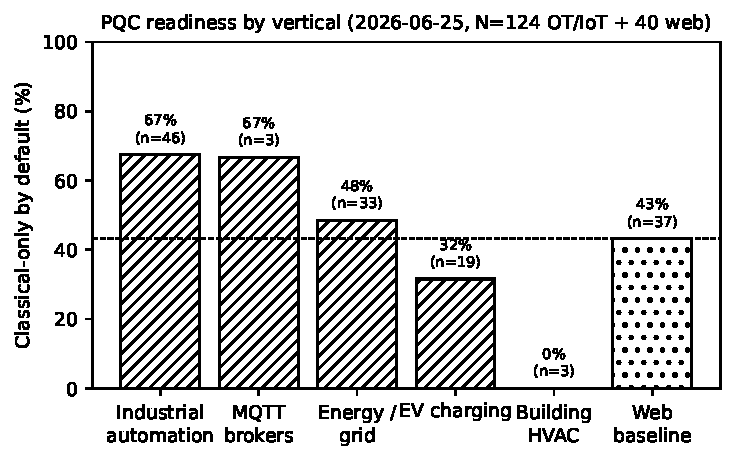
\includegraphics[width=0.86\linewidth]{figures/verticals.pdf}
\caption{Default classical-only rate by vertical, computed directly from the
released scan results. Bars are labelled with the resolvable sample size per
vertical; the dashed line marks the 43\% web baseline. Industrial-automation
vendors are the only vertical materially above the web baseline.}
\label{fig:verticals}
\end{figure}

Figure~\ref{fig:verticals} plots the per-vertical rates in
Table~\ref{tab:otiot}; the vertical ordering makes the single clear signal
visible: industrial automation is the lone laggard, while EV-charging and
building-HVAC sit below the web baseline.

\paragraph{Findings.}
\begin{itemize}
  \item \textbf{Industrial-automation vendors are the laggard vertical: 67\%
        classical-only by default} (31/46 resolved), markedly above the 43\% web
        baseline and the highest of any vertical. The classical-only cohort includes
        \textbf{Siemens, Schneider Electric, Honeywell, ABB, GE Vernova, Bosch Rexroth,
        Fanuc, Keyence, Festo, Phoenix Contact, SICK, Endress+Hauser, Pepperl+Fuchs,
        Lenze, Danfoss, Parker, ifm, Weidm\"uller, Moxa, Hitachi Energy, Red Lion,
        Lantronix, AspenTech, Inductive Automation} and more. Migrated automation
        vendors were the minority (Emerson, Beckhoff, WAGO, Pilz, Turck, HMS, Advantech,
        Yaskawa, Digi, \ldots).
  \item \textbf{EV-charging leads the web (32\% classical):} consumer portals are
        CDN-fronted and largely migrated; classical-only were Tesla, Blink, EVBox,
        Alfen, GridServe. Migration tracks the front-end CDN, not the sector.
  \item \textbf{Energy/grid mirrors the web (48\%):} migrated (National Grid, ISO-NE,
        Southern Co, Dominion, Enel, E.ON, MISO, ERCOT, TenneT, Xcel, ConEd, SCE,
        \ldots) vs.\ classical-only (Duke, US \code{eia.gov}, EU \code{entsoe.eu},
        PSEG, NextEra, EDF, Iberdrola, Vattenfall, RTE, Terna, \ldots).
  \item \textbf{Building automation (HVAC) is fully migrated} (Johnson Controls, Trane,
        Carrier; 3 of 3), a clean contrast with industrial automation.
  \item \textbf{PQC reaches real IoT protocol endpoints:}
        \code{test.mosquitto.org:8883} negotiated \code{X25519MLKEM768}
        (\code{broker.emqx.io} and \code{mqtt.flespi.io} were classical-only). Hybrid
        key exchange is viable on MQTT-over-TLS today.
\end{itemize}

\paragraph{Reading.}
The gap is \textbf{vertical-specific, not blanket}. The early small-sample ``OT lags
everywhere'' hypothesis did not survive scaling: EV-charging and building-HVAC
actually lead the web, and energy matches it. What holds, and stays stable from
$N{=}24$ (71\%) through $N{=}46$ (67\%) resolved vendors, is that
\textbf{heavy-industrial automation vendors lag markedly (${\sim}67\%$
classical-only)}, which is the concrete, defensible contribution. The deeper
device/control-plane exposure (RTUs, PLCs, OCPP central systems) remains unmeasurable
from the public Internet; quantifying it requires operator or laboratory access,
which is precisely the follow-on research program this measurement motivates.

\subsection{Longitudinal stability (first re-scan, T0 + 7 days)}
\label{sec:longitudinal}

We re-ran the identical probe (same host lists, same 8\,s single-vantage
methodology, same OpenSSL 3.5.6 build) on 2026-07-02, seven days after the
baseline, to separate real migration movement from measurement noise.

\begin{table}[h]
\centering
\begin{tabular}{lccc}
\toprule
Population & Hosts compared & Verdict unchanged & Migrations observed \\
\midrule
OT/IoT ($N{=}124$) & 124 & 123 (99.2\%) & 0 \\
Web ($N{=}40$)     & 40  & 40 (100\%)   & 0 \\
\bottomrule
\end{tabular}
\caption{Longitudinal re-scan, 2026-06-25 $\rightarrow$ 2026-07-02. The single
changed verdict (\code{aspentech.com}: classical-only $\rightarrow$ unknown)
returned no negotiated group within the probe window, a vantage/timeout
artifact rather than a class change.}
\label{tab:longitudinal}
\end{table}

\begin{figure}[h]
\centering
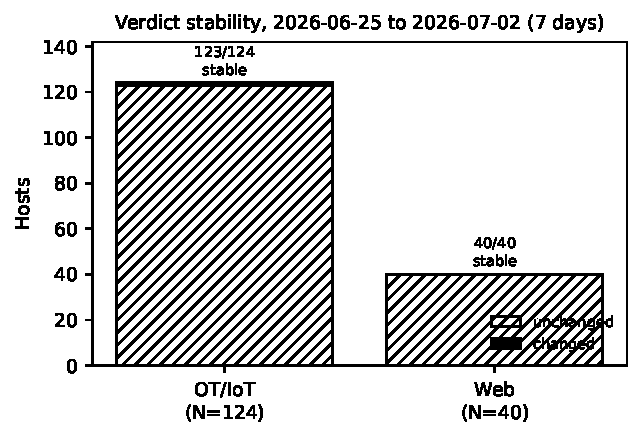
\includegraphics[width=0.62\linewidth]{figures/longitudinal.pdf}
\caption{Verdict stability across the two runs, computed from the released
baseline and re-scan JSON. 163 of 164 host verdicts are identical one week
apart.}
\label{fig:longitudinal}
\end{figure}

Two things follow (Table~\ref{tab:longitudinal}, Figure~\ref{fig:longitudinal}).
First, verdict stability of 99.4\% (163/164) across independent runs a week
apart is direct evidence that the single-vantage handshake classification is
reproducible rather than a per-connection artifact. Second, no endpoint in
either population migrated to post-quantum key exchange over the interval:
every classical-only host at the baseline, including the industrial-automation
cohort and the cryptography-authority sites, remained classical-only. At this
cadence, OT/ICS PQC migration is effectively flat week-to-week, which sharpens
the long-exposure-window concern that motivates the study. We will continue the
re-scan on a monthly cadence to recover the migration slope.

\paragraph{Next steps.}
Continued longitudinal re-scans to chart the migration slope; lawful
device-plane endpoints via disclosure partners; multi-vantage probing to
recover the 20 unresolved hosts.

\section{Ethics and Responsible Disclosure}
\label{sec:ethics}

\begin{itemize}
  \item Handshake-only; no payloads, no denial of service, no exploitation. Load is
        equivalent to a single browser connection per probe.
  \item Public, owner-operated endpoints only; abuse contacts honored; rate-limited.
  \item Named high-value classical-only sites are disclosed privately before
        publication where appropriate.
  \item The released dataset contains only hosts that are already public
        infrastructure; no credentials, no personal data.
\end{itemize}

\section{Limitations}
\label{sec:limits}

\begin{itemize}
  \item Single network vantage point: middleboxes and anycast can yield \code{UNKNOWN}
        or vantage-specific results (3/40 in the web baseline). Multi-vantage scanning
        is planned.
  \item Default negotiation depends on the client's offered preference order; we fix it
        and document it.
  \item The $N{=}40$ web baseline is illustrative, not representative; the contribution
        rests on the OT/IoT vertical (\S\ref{sec:otiot}), not the web $N$.
  \item Point-in-time snapshot; migration is moving, and the longitudinal scan addresses
        this.
\end{itemize}

\section{Conclusion}

PQC migration is real but front-end-driven and deeply uneven: even NIST's and OpenSSL's
own sites, and cryptography universities, were classical-only at scan time. The
consequential gap is in OT/IoT/critical-infrastructure endpoints, where
industrial-automation vendors lag at ${\sim}67\%$ classical-only against a 43\% web
baseline. We release the scanner and dataset to make PQC-readiness a continuously
measurable property rather than an assumption.

\paragraph{Artifacts.}
Scanner: \url{https://github.com/s-shahzad/pqc-readiness-scanner} (\code{pqc\_scan.py},
MIT license). Datasets: \code{scan-results.json} (web baseline),
\code{seed-ot-iot\{,-2,-3\}.json} (OT/IoT scans, 2026-06-25),
\code{rescan-\{ot-iot,web\}-2026-07-02.json} (longitudinal re-scan), with the
per-run comparison in \code{LONGITUDINAL.md}. Figures are regenerated from these
files by \code{make\_figures.py}.

\begin{thebibliography}{9}

\bibitem{fips203}
National Institute of Standards and Technology.
\newblock Module-Lattice-Based Key-Encapsulation Mechanism Standard.
\newblock FIPS 203, August 2024.

\bibitem{mosca2018}
M. Mosca.
\newblock Cybersecurity in an era with quantum computers: Will we be ready?
\newblock \emph{IEEE Security \& Privacy}, 16(5):38--41, 2018.

\bibitem{ietfmlkem}
K. Kwiatkowski, P. Kampanakis, B. Westerbaan, and D. Stebila.
\newblock Post-quantum hybrid ECDHE-MLKEM key agreement for TLSv1.3.
\newblock IETF Internet-Draft, draft-ietf-tls-ecdhe-mlkem, work in progress.

\bibitem{zmap}
Z. Durumeric, E. Wustrow, and J. A. Halderman.
\newblock ZMap: Fast Internet-wide scanning and its security applications.
\newblock In \emph{USENIX Security Symposium}, 2013.

\bibitem{censys}
Z. Durumeric, D. Adrian, A. Mirian, M. Bailey, and J. A. Halderman.
\newblock A search engine backed by Internet-wide scanning.
\newblock In \emph{ACM CCS}, 2015.

\bibitem{paquin2020}
C. Paquin, D. Stebila, and G. Tamvada.
\newblock Benchmarking post-quantum cryptography in TLS.
\newblock In \emph{PQCrypto}, 2020.

\bibitem{sikeridis2020}
D. Sikeridis, P. Kampanakis, and M. Devetsikiotis.
\newblock Post-quantum authentication in TLS 1.3: A performance study.
\newblock In \emph{NDSS}, 2020.

\bibitem{ibrahim2026raw}
M. Ibrahim, V. Ajith, and M. S. Haroon.
\newblock Detecting post-quantum and hybrid TLS deployments via raw TLS record
inspection.
\newblock Cryptology ePrint Archive, Paper 2026/834, 2026.

\bibitem{delgado2026observability}
J. L. Delgado.
\newblock Observability for post-quantum TLS readiness: A multi-surface evidence
framework.
\newblock Cryptology ePrint Archive, Paper 2026/866, 2026.

\bibitem{albrecht2024wild}
M. R. Albrecht and K. G. Paterson.
\newblock Analysing cryptography in the wild.
\newblock Position paper, 2024.

\bibitem{westerbaan2024state}
B. Westerbaan.
\newblock The state of the post-quantum Internet.
\newblock Cloudflare blog, 2024. \url{https://blog.cloudflare.com/pq-2024/}.

\bibitem{rfc9528}
G. Selander, J. Preu{\ss} Mattsson, and F. Palombini.
\newblock Ephemeral Diffie-Hellman over COSE (EDHOC).
\newblock RFC 9528, 2024.

\bibitem{mqtt5}
OASIS.
\newblock MQTT version 5.0.
\newblock OASIS Standard, 2019.

\bibitem{ocpp201}
Open Charge Alliance.
\newblock Open Charge Point Protocol 2.0.1.
\newblock 2020.

\bibitem{shaik2025ocpp}
A. S. Shaik, M. Gutla, A. P. R. Kagitala, and S. Bhatia.
\newblock Plugged-in and protected: Leveraging machine learning to secure IoT-based
electric vehicle charging stations from denial-of-service threats.
\newblock In \emph{IEEE Global Conference on Artificial Intelligence and Internet of
Things (GCAIoT)}, 2025. DOI: 10.1109/GCAIoT68269.2025.11275540.

\end{thebibliography}

\end{document}
